\documentclass[]{proc}
%\documentclass[•]{article}
\usepackage[utf8]{inputenc}
%\usepackage[ngerman]{babel}
\usepackage{eurosym}
\usepackage{import}
\usepackage{graphicx}
\usepackage{tikz}
%\usepackage{listings}
\usepackage{url}
\usetikzlibrary{arrows,automata}
\begin{document}
\title{OpenJukebox}
\author{Benjamin Fus}
\maketitle
\tableofcontents
\begin{abstract}
	There are several network player on the market, which all based on proprietary software. Because of this proprietary the network player is mostly uncomfortable in use and it is not usable from every network device. To improve this weakness the goal of this project is to build a network player which is controllable via the Music Player Daemon (MPD). MPD uses a extreme simple protocol which based on ascii Strings. This simple protocol allows to interact via a telnet client with the mpd server. The network player will get a own hard drive and will be able to play internet radio and audio from other sources.
\end{abstract}
\section{Hardware}
Existing development boards has been chosen to build the network player with a minimal  effort of development. The power supply will be build in a classic way with a toroidal transformer, bridge rectifiers and a reservoir capacitor. After this simple power supply two different voltages will be provided by two step-down transformer. The core of the network player will be a Carambol2 2.
\subsection{Carambola2}
The Carambola2 is a System On Chip (SoC) Module which has a MIPS processor with 400 MHz clock, 16 MB of SPI-Flash and 64 MB of RAM. The SoC provides 2 Ethernet connectors and a Wifi module as well as UART access and buses like inter circuit communication (i2c). Especially for audio playback the Carambola2 is equipted with the Inter-IC Sound(i2s) bus which is a bus for serielle digital audio transmission as well as Sony/Philips Digital Interface (S/PDIF) which is a interface specification for a digital audio interface for stereo or multi-channel audio. Unfortunately, there is no driver to use either i2s nor S/PDIF under openWRT because of this a USB sound card must be used to provide an audio output.
\begin{figure}[h!]
\begin{center}
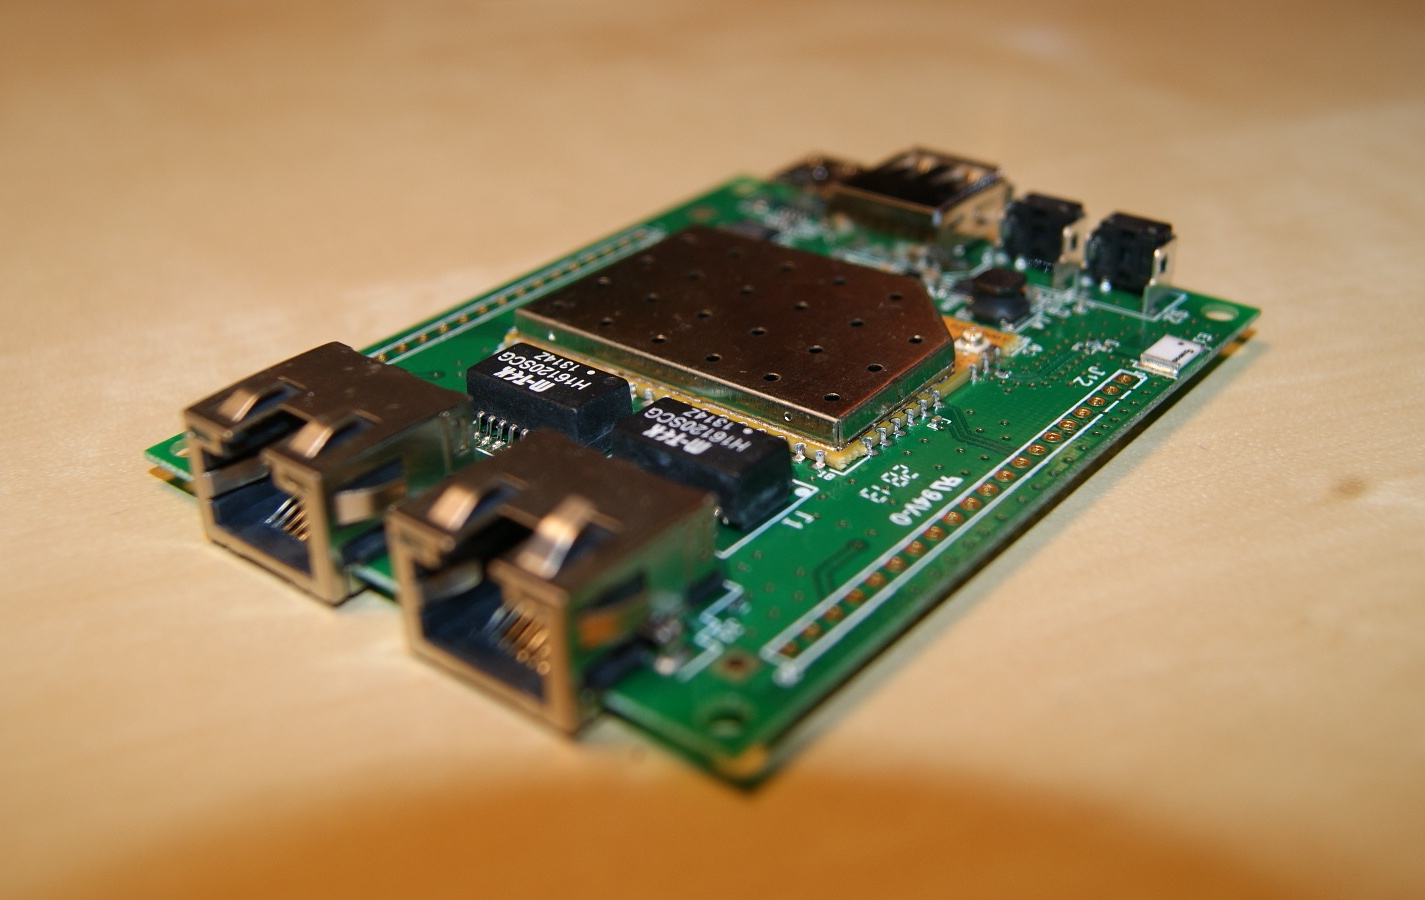
\includegraphics[scale=0.4]{pictures/carambola2}
\caption{Carambola2}
\end{center}
\end{figure}
\subsection{USB-Sound}
In the selection of the chipset for the USB-Soundchip the choice falls on the PCM2704 from Texas Instruments.The PCM2704 provides direkt analog audio output via Burr Brown Digital Analog Converter as well as digital audio output over S/PDIF and Toslink. In this case the referencedesing for the PCM2704 is available as an development board and that is used in this project. The PCM2704 operates directly as Human Interface Device(HID) which means that no special driver is needed. If there is a driver for the Carambola2 i2s and SPDIF available in the future, this hardware component will be obsolete.

\begin{figure}[h!]
\begin{center}
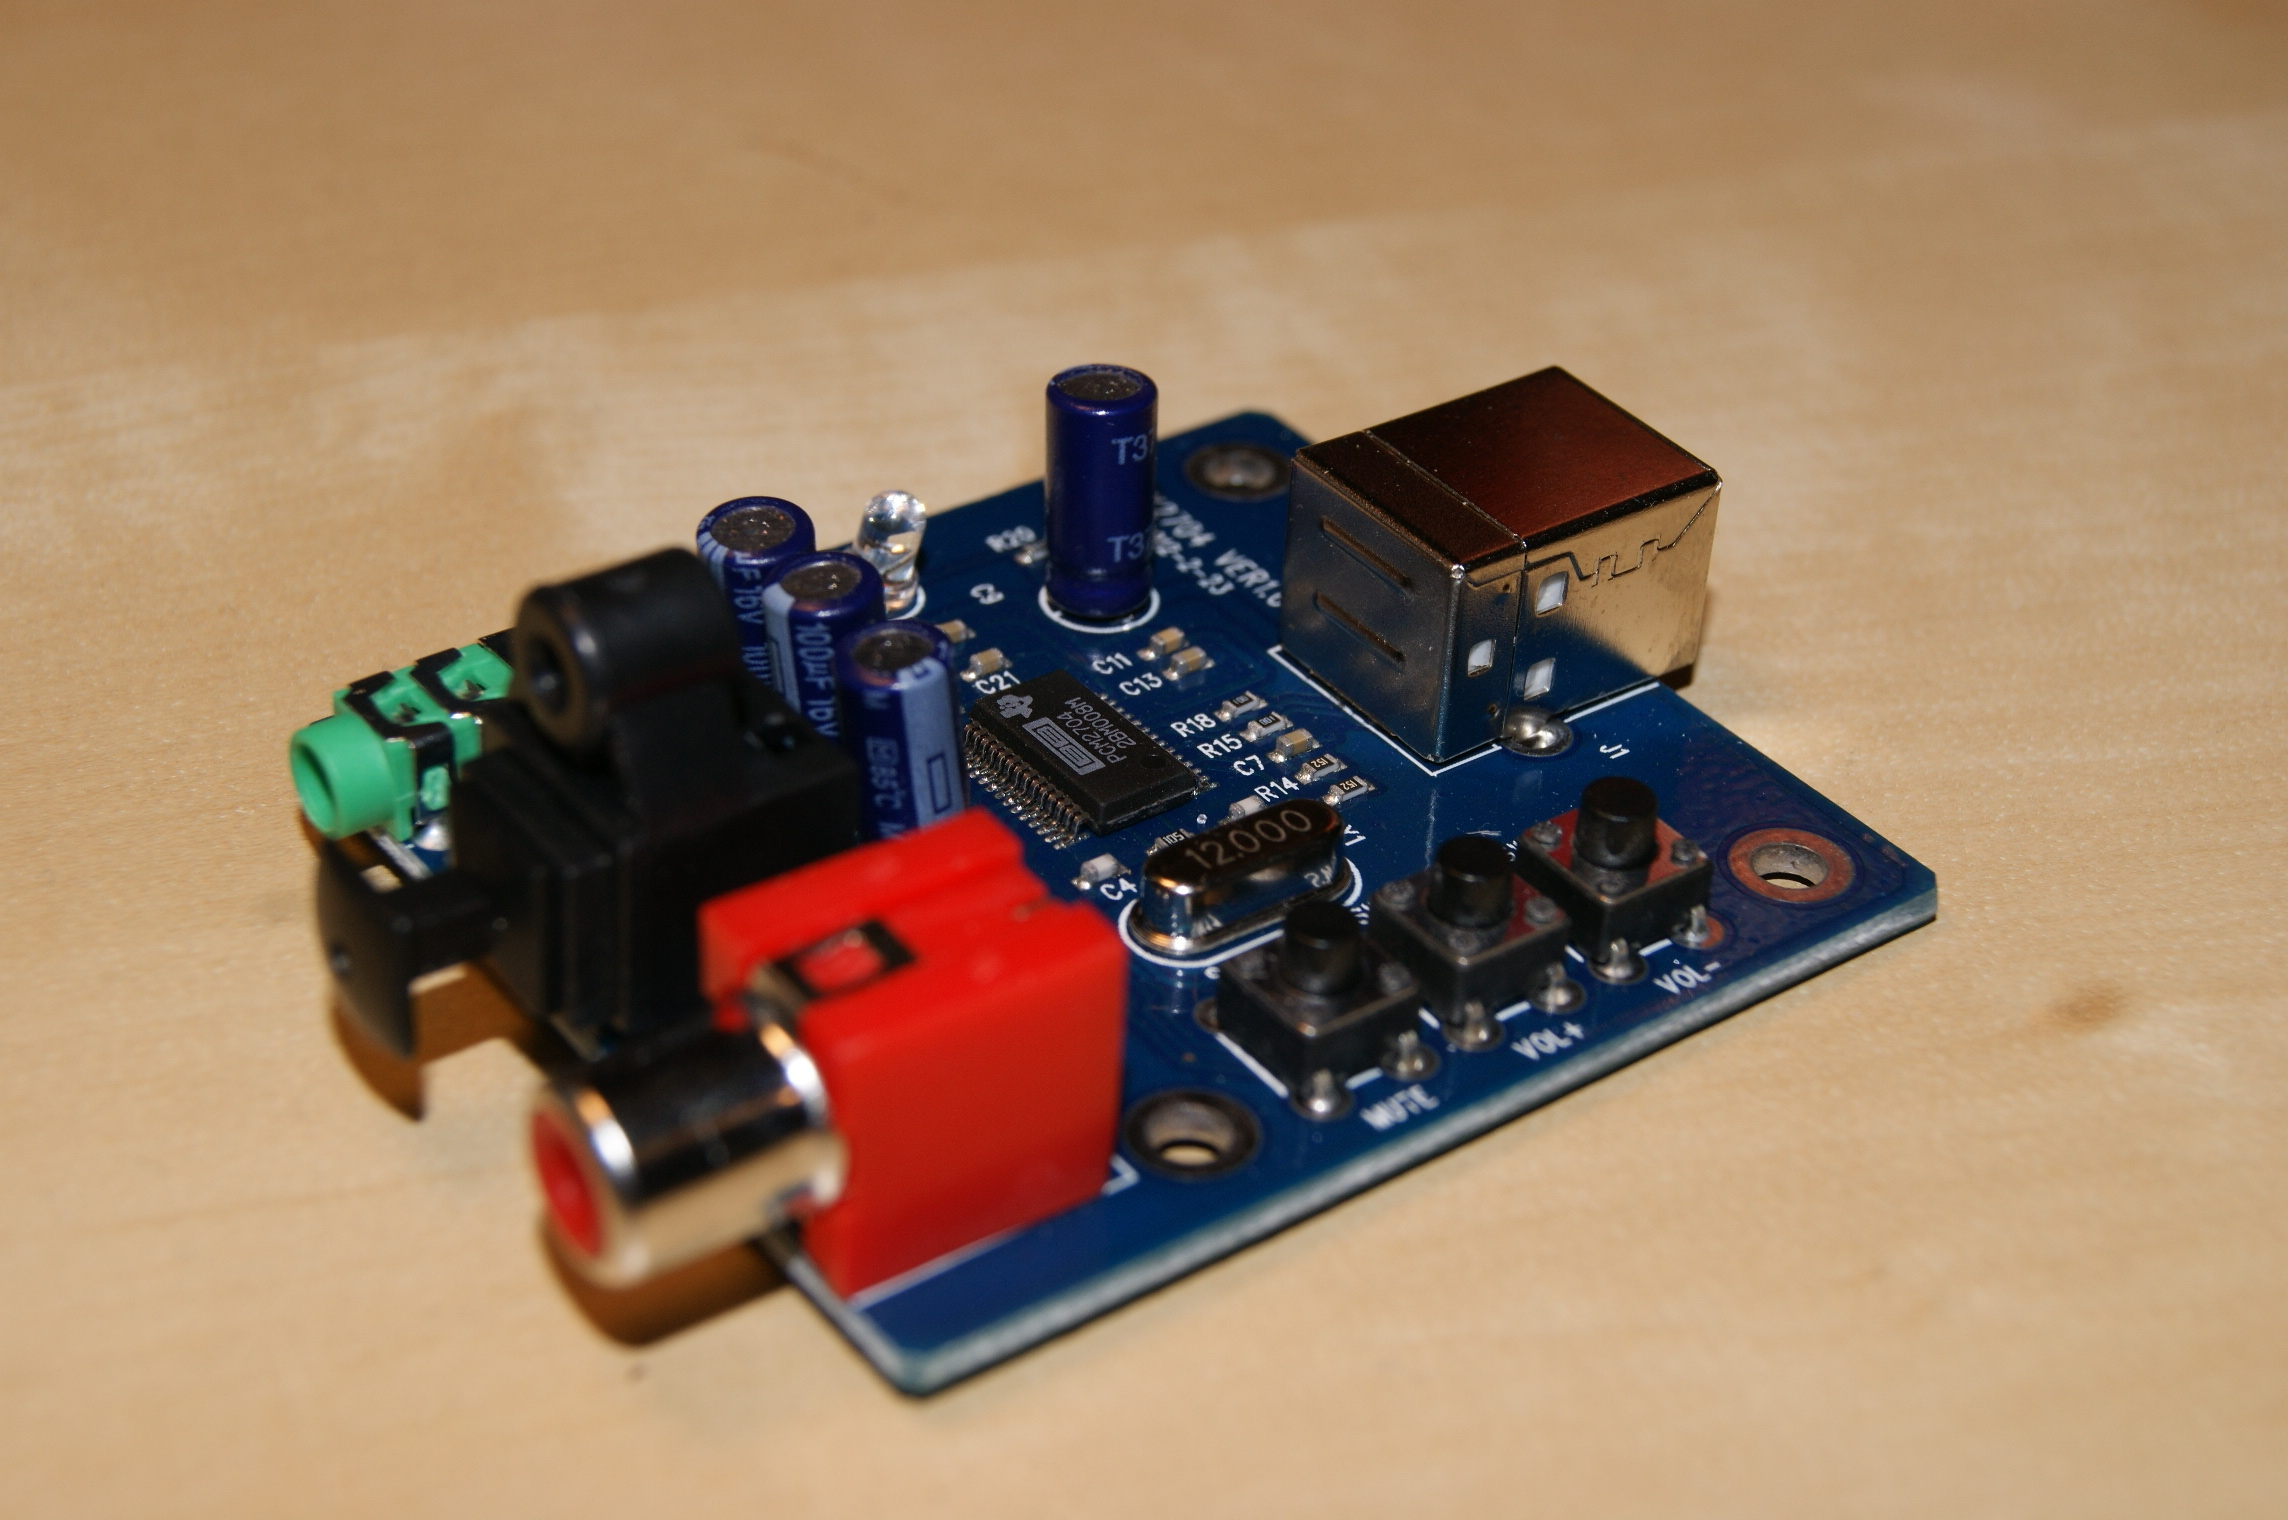
\includegraphics[scale=0.35]{pictures/pcm2704}
\caption{PCM2704}
\end{center}
\end{figure}
\subsection{LCD-Display}
To display informations like title or artist there will be used a common lcd display with a hd4478 chipset with 16 columns and 2 rows or 20 clumns and 4 rows. To controll the display the circuit "LCD2USB" from Dr. Till Harbaum will be used. This circuit consist of an Atmel ATMEGA8 and uses the Avrusb library to communicate directly via USB with the LCD display. As alternative we will test a circuit which controls the LCD display via i2c. This has the advantage that the USB hub has one device less to manage.
\subsection{Power supply}
Goal of the power supply is to provide the internal voltage with a minimum of noise.The power supply is designed in a classic way with an toroidal transformer and step-down transformer to provide 5V and 3.3V as output voltage. In the first step the torodial transformer transforms the 220V alternating current voltage into 12V alternating current voltage which feeds an bridge rectifier to get direct current voltage. The direct current voltage from the bridge rectifier fluctuate. To smooth the voltage a reservoir capacitor is used. The capacity of the capacitor can be calculated with the following formula.


\begin{equation}
	C=I*\frac{\Delta t}{\Delta U}
	\label{reservoidCapacitor}
\end{equation} 

In this case $\Delta t$ stands for the netfrequency diviced by two which means at a 50Hz we have $\Delta t = 10ms$. $\Delta U$ stands for the amount of voltage which can be lost during $\Delta t$.The toroiadal transformer can provice a current of 2.5A. 
\begin{center}
	$C=2.5A * \frac{10*10^-3s}{0.1V}=0.25F$
\end{center}
Because we use half-wave rectification the capacity must be doubled. The reservoir capacitor must have 0.5F


\subsection{Front panel control}
As input device will be used a rotary encoder on the front panel.

\section{Software}
\subsection{OpenWRT}
\subsubsection{Patch for MPD-full}
If the compilation of OpenWRT fails at the mpf-full package it is necesarry to patch the package with this \footnote{\url{http://patchwork.openwrt.org/patch/4335/}}{patch}. This patch is commited on the OpenWRT mailinglist but acceptet till today.
%\lstinputlisting[caption=mpd-patch, language=make]{../openWRT-patches/OpenWrt-Devel-packages-sound-mpd-update-to-mpd-0.16.8.patch}


%\section{Housing}
The housing gets the dimensions of an average hifi case to fit in an old hifi rack.
The actual dimensions are
\begin{itemize}
	\item Height: 10cm
	\item Width: 43,5cm
	\item Depth: 30cm
\end{itemize}
\listoftables
\listoffigures


\end{document}